\section{Background}
\label{S:Back}

\subsection{State of the Art}
\label{SS:Back:SOA}
    
In the literature there are two problems that are often addressed when dealing with MRSLAM:
\begin{enumerate}
\item robot coordination, i.e., how to cover the most area given an unknown environment \cite{julia2012comparison}, and
\item merging the data to create one global map posterior, which is what we will focus on.
\end{enumerate}

In the case where all relative robot poses are known, merging maps is a trivial problem using small modifications to existing SLAM techniques \cite{thrun2001probabilistic}. In the general MRSLAM problem, however, robots may start with unknown absolute and relative poses, and therefore merging of maps requires the discovery of relative relationships between different robot trajectories to build a single map. This is often a costly process, which in general can be solved for robots sharing a search space by estimating each robot's relative pose given a partial map, but this leads to exponential complexity with respect to the number of exploring robots \cite{fox2006distributed}. Nevertheless, several practical algorithms exist to circumvent this naive and inefficient approach,  including coarse topological matching and stitching techniques borrowed from computer vision \cite{birk2006merging}.

In 2006 two schools of thought arouse about how to handle MRSLAM:
\begin{enumerate}
\item Let independent robots build individual maps, then at the end combine the maps together \cite{birk2006merging}.  This approach is particularly attractive for post processing because it requires multiple trial and error to maximize a score function. 
\item On the other hand, there was Howard's paper \cite{howard2006multi}, which uses communication between robots, but requires precisely known relative poses to construct a single global map posterior.
\end{enumerate}
Both had their benefits: \cite{birk2006merging} does not require knowledge of any global or relative poses, but \cite{howard2006multi} can be implemented in real-time.  Because of the real-time nature, and the desire to map as fast as possible, there has also been a great deal of research using \cite{howard2006multi}, but with the added constraint of limited communication \cite{lazaro2013multi}.

In the following subsection we will propose yet another extension to \cite{howard2006multi}.

\subsection{Extension of \cite{howard2006multi}}
\label{SS:Back:Contributions}


Define the weights for a particle filter: $w_t^i$, and the sensor model, $p(z_t|\textbf{x}_t,u_{t-1})$ for the forward and reverse model.  In \cite{howard2006multi}, Howard follows the typical RBPF formulation and defines the un-normalized weight update to be:
\begin{equation}
w^{(i)}_t=p(z_{t}^{f}|\textbf{x}_{t}^{f(i)},m_{t-1}^{(i)}) p(z_{t}^r|\textbf{x}_{t}^{r(i)},m_{t-1}^{(i)}) w^{(i)}_{t-1},
\label{eq:combinedweight}
\end{equation}
where $\bullet^{f(i)}$ and $\bullet^{r(i)}$ denote the forward and reverse elements of particle $(i)$, $\textbf{x}_{t}$ denotes the pose, $z_{t}$ denotes the measurement, and $m_{t-1}$ denotes the map..

In this formulation it is no stretch of the imagination that the forward sensor model and previous weight $p(z_{t}^{f}|\textbf{x}_{t}^{f(i)},m_{t-1}^{(i)}) w^{(i)}_{t-1}$ could be large, denoting a good match to the data in the forward direction, yet the reverse sensor model, $p(z_{t}^{r}|\textbf{x}_{t}^{r(i)},m_{t-1}^{(i)})$, could be small.  Thereby reducing the probability that the best forward direction is resampled.  See for example Fig. \ref{fig:deplete}, particularly particle 1.


Because of this, we propose assuming that the noisy forward and reverse motions are independent, motivates using two particle filters with weights defined by:
\begin{eqnarray}
w^{f(i)}_{t}&=&p(z_{t}^f|\textbf{x}_{t}^{f(i)},m_{t-1}^i)  w^{f(i)}_{t-1}\\
w^{r(i)}_{t}&=&p(z_{t}^r|\textbf{x}_{t}^{r(i)},m_{t-1}^i)  w^{r(i)}_{t-1}
\end{eqnarray}
and with $\{\textbf{x}_{t}^{f(i)},m_{t-1}^i\}$ being resampled using $\{w^{f(i)}_{t}\}$, and $\{\textbf{x}_{t}^{r(i)}\}$ being resampled using $\{w^{r(i)}_{t}\}$.  


\begin{figure}[h]
\centering
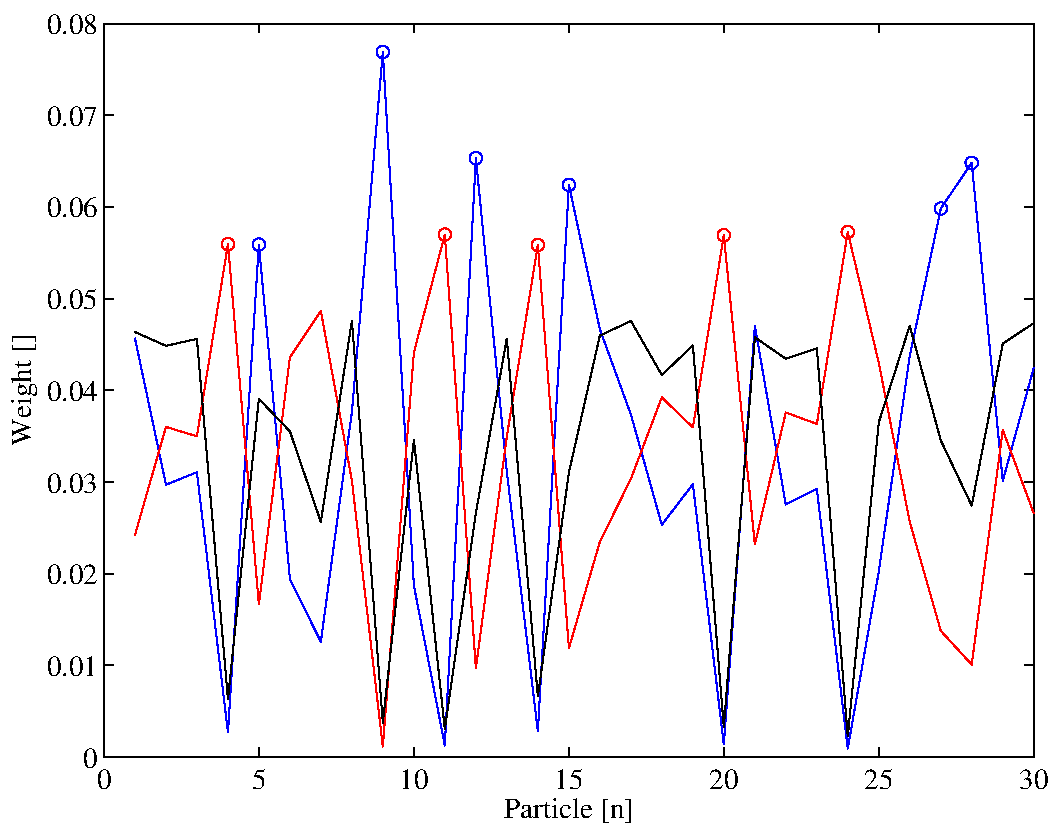
\includegraphics[width=\columnwidth]{../FinalFigures/Depletion}
\caption{Case where the best forward and reverse poses are not chosen. $w^{f(i)}_{t}$ is the forward weight, $w^{r(i)}_{t}$ is the reverse weight, and $w^{(i)}_t$ is the product of the weights.}
\label{fig:deplete}
\end{figure}

Our contribution is two-fold, verifying that Howard's algorithm works, and creating independently sampled particle filters for each mapping robot in the aim to build a more accurate occupancy grid, and obtain a better localization within the map while only marginally increasing the computational complexity.

